
\begin{figure}[H]
\caption{The Four-Stage Learning Cycle by Kolb (1984)}\label{fig:exp4stages}
\centering
\centering
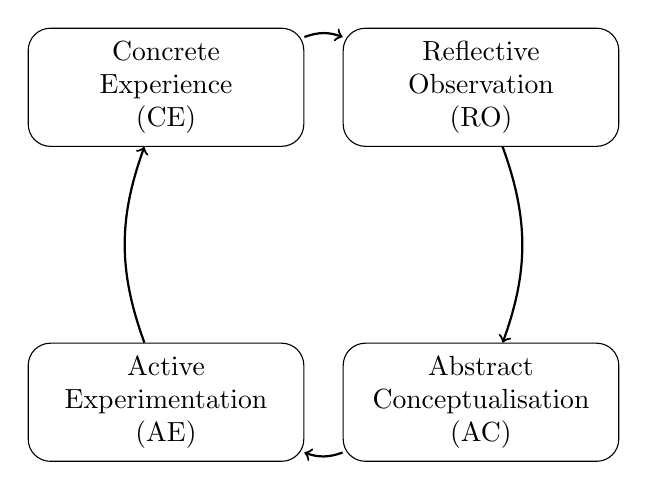
\begin{tikzpicture}[
    node distance=4cm,
    every node/.style={
        draw,
        rounded corners=8pt,
        minimum width=3.5cm,
        minimum height=1.5cm,
        align=center
    },
    arrow/.style={->, thick}
]

% Nodes
\node (ce) {Concrete\\Experience\\(CE)};
\node (ro) [right of=ce] {Reflective\\Observation\\(RO)};
\node (ac) [below of=ro] {Abstract\\Conceptualisation\\(AC)};
\node (ae) [left of=ac] {Active\\Experimentation\\(AE)};

% Arrows
\draw[arrow] (ce) to[bend left=20] (ro);
\draw[arrow] (ro) to[bend left=20] (ac);
\draw[arrow] (ac) to[bend left=20] (ae);
\draw[arrow] (ae) to[bend left=20] (ce);

\end{tikzpicture}
\end{figure}
